 \subsection{Request of selected data of a specific user with subscription and data visualization}
 
The Third Party can exploit the Data4Help System, sending a request for the selected data (health data and location) of a specific User, either the last available data, or in subscription mode.  
In the latter case it inserts the interval time, i.e. how often wants to receive the updates of these data.
The User can manage his requests, and decide to accept or deny them. If the request is authorized, the Third Party receives the requested data from the System, according to the chosen modalities.

\begin{table}[H]
	\centering
    
    \begin{tabular}{|p{3.5cm}|p{10.3cm}|}
    
    \hline
    \textbf{\large{Actors}}  			& \tabitem Third Party \\
                                        & \tabitem  User \\
    				 			
    \hline
    \textbf{\large{Goals}} 				&\ref{goal:user1} \ref{goal:parties1} \ref{goal:parties2} \ref{goal:parties3} \ref{goal:parties7}\\
    
    \hline
    \textbf{\large{Enter Condition}} & The Third Party is already logged in.\\
    
    \hline
    \textbf{\large{Events Flow}}		& \begin{enumerate}[leftmargin=0.5cm]
                                            \item The \emph{Third Party} selects the Individuals section.
                                          	\item The \emph{Third party}  presses the "New Request" button.
                                            \item The \emph{Third party} inserts the specific fiscal code of the target User.
                                            \item The \emph{Third party} specifies the data that want to receive.
                                            \item The \emph{Third Party} can select the subscription mode. If 
                                        it is chosen, the \emph{Third Party} should also specify the interval time for receiving updates.
                                            \item The System sends an authorization request to the target User with all the related informations.
                                            \item  The \emph{User} receives the request in his "Inbox" section and can decide to accept or deny it.
                                            \item If the request is accepted, the System retrieves the requested data. (If the \emph{Third Party} has performed a subscription request, the System sends the updates to the \emph{Third Party} how often it has requested).
                                            \item The requested data are shown to the \emph{Third Party}.
                                
                                          \end{enumerate}
    										\\
    \hline
    \textbf{\large{Exit Condition}} 	& The Third Party can examine the requested data. \\
    
    \hline
    \textbf{\large{Exception}} 			& \begin{enumerate}[leftmargin=0.5cm]
                                          	\item The target \emph{User} denies the request: the negative response is communicated to the \emph{Third Party}.
                                          	\item The selected fiscal code does not correspond to a registered \emph{User}:the System asks to insert a validate one.
	\end{enumerate}\\
    
    \hline
    
    \end{tabular}
	
\end{table}

\begin{figure}[H]
    \centering
    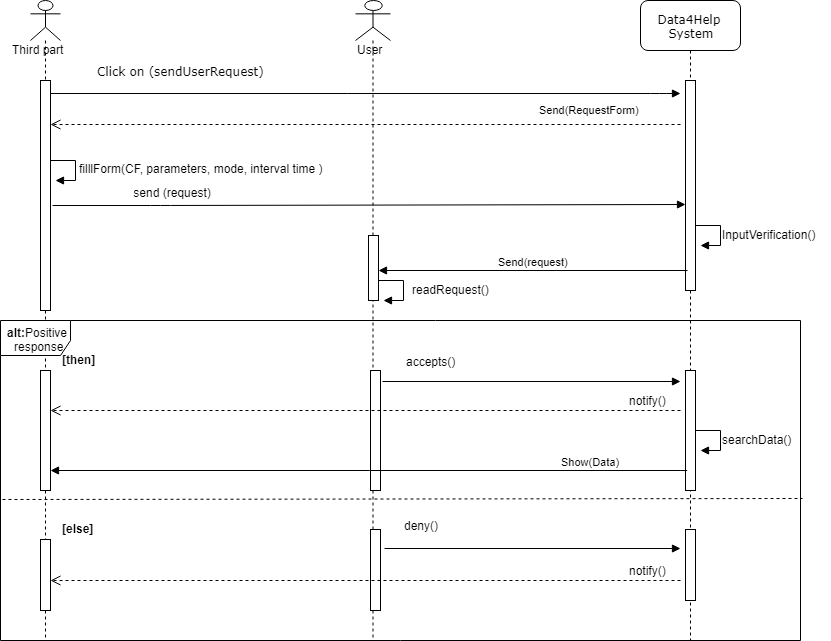
\includegraphics[scale=0.4]{rasdL/Pictures/request1.png}
    \caption{Sequence diagram for requesting data of a specific User}
  
\end{figure}